\documentclass[12pt]{article}

\usepackage{amsmath}
\usepackage[margin=1in]{geometry}
\usepackage{graphicx}
\graphicspath{ {/} }
 

\makeatletter
\def\l@section{\@dottedtocline{1}{0em}{3em}}
\makeatother

\begin{document}

\title{An Introduction to Cost Estimation of Relational Query Plans}
\author{Yannis Velegrakis}

\maketitle

\tableofcontents

\section{Page}

Every time a hard drive is instructed to read or write something on the disk it does so by reading or writing units of specific size. This size is called a PAGE and has always a fixed size for every system. For example, if the page size is 1024 bytes and the database wants to read 3 bytes from the disk, the disk will read and return to the database 1024 bytes of which the database will throw away the 1021 and keep only the needed 3.
The size of a page on the disk will be denoted as $P$.

\section{Size of a Record}

We assume that the records of a relation have more or less the same size. The size of a record indicating how much space (in bytes) a record occupies when stored on the disk. The size of a record will be typically given, or if not, it would be possible to compute from the size of the individual attributes. For example, if a relation has five attributes, three of them being integers and two being VARCHAR(25), then the size of a record for this relation is 3*4+2*25=62 bytes. The size of a record of a relation R will be denoted as $t_R$.

\section{Pages of Relations}

The data of every relation are stored on the disk. When a page contains some data of a relation, no records from other relations are allowed in that page. What the databases try to do is to try to fill a page with as many records of the same relation as they can, and if no more records can fit, then they start with another page. This means that we can safely assume that all the pages that a relation occupies on the disk are full.
The number of pages that a relation R occupies on the disk will be denoted as $P_R$.

\section{Cardinality of a Relation}

A relation is a set of records. The number of records a relation has is the cardinality of the relation. The cardinality of a relation R will be denoted as $|R|$.

\section{Cardinality of an Attribute}

The cardinality of an attribute in a relation is the number of different distinct values that the attribute has. If the attribute is a key, clearly the cardinality of the attribute is the same as the cardinality of the relation, i.e., the number of records of the relation (since a value cannot be repeated). \\
The cardinality of two or more attributes is similarly the number of different distinct combinations of values of these attributes across the records.
The cardinality of an attribute A of a relation R, will be denoted as $|R.A|$, and the cardinality of two or more attributes as $|R.A_1, R.A_2, ..., R.A_n|$. So, if the attribute A is a key, then $|R| = |R.A|$, otherwise $|R.A| \le |R|$.

\section{Records per Page}
The database does not store in the same page records from different relations. Furthermore, the database does not store a record across different pages. For instance, if a page size is 100 bytes and a record has a size of 30 bytes, then only 3 records will fit in a page (taking space 3*30=90 bytes), and the remaining 10 bytes from the 100 will be left empty. This means that

$$
\text{\#Records of R per Page} = \Big\lfloor\frac{\text{Page Size}}{\text{Tuple Size of R}}\Big\rfloor = \Big\lfloor\frac{P}{t_R}\Big\rfloor
$$

The symbol $\lfloor \rfloor$ means that we round down to the closest integer. So if the division gives 4.3, then the number of records per page will be 4.

\section{Relation Size}

The size of a relation is the space it occupies on the disk. Since there are spaces left in pages, that size is often more than the actual size of its records. So, the size of R in bytes is:

$$
\text{Size of R} = \text{\#Pages of R} * \text{PageSize} = \Big\lfloor\frac{\text{\#Tuples of R}}{\text{\#Tuples of R per page}}\Big\rfloor P \\
= \Big\lfloor\frac{ |R| }{\lfloor\frac{P}{t_R}\rfloor}\Big\rfloor P
$$

The symbol $\lceil \rceil$	means that we round up to the closest integer. So, if the internal part is 4.3, then the $\lceil \rceil$ will be 5.
From the above mathematical equation, it becomes clear that:

$$
|R| = P_R * \#\text{of records of R in a page} = P_R * \Big\lfloor\frac{P}{t_R}\Big\rfloor
$$

\section{Cost}

Operations that involve reading from the disk or writing to the disk are called I/O. Operations that are done only in memory are called in-memory. The cost of an in-memory operations is so much smaller than that of an I/O that it is the number of needed I/O operators that are actually determining the cost (time) that a query will take to be executed. For this reason, we will consider the cost of any inmemory operation to be 0 (zero) and we will measure the cost of the execution of a query in terms of number of I/O operations. By definition we will assume that the cost of reading or writing a page on the disk is equal to 1.

\section{Scan}

A scan operation is a sequential read of a relation. The cost is the cost of reading all the pages that the relation occupies. Thus,

$$
\text{Cost of Scan} = \#\text{Pages of the relation}
$$

For the database to find and read a record in a relation normally it needs to do a scan since the record can be in any of the pages that the relation occupies, and in the absence of any auxiliary structure (for instance the indexes we will see later) or any special organization of the data (for instance if the data is sorted), then the scan is the only option.

\section{Sorting}
If we need to sort a relation based on the value of a specific attribute, there are two main algorithms that this can be done. One of these algorithms assumes that the database has only 3 buffers in its memory. If N is the number of pages occupied by the relation that needs to be sorted, the cost of the sorting (in terms of required I/O operations) is:

$$
2N(\lceil \log_2(N)\rceil + 1)
$$


Typically, a database has more than 3 memory buffers available for sorting, so an optimized algorithm can be used. If there are B available buffers (with B>3), then the cost of sorting a relation that occupies N pages (in terms of required I/O operations) is:

$$
2N(\lceil \log_{B - 1}(\lceil\frac{N}{B}\rceil)\rceil + 1)
$$

The details of the algorithms can be found in the course textbook, but for us it is enough to simply know these two algorithms and the cost that each one has.

\section{Indexes}

An index is an auxiliary structure that is built based on the values of a specific attribute of the database. It helps in identifying the location of the records (meaning the pages in which they reside) that have a value in that attribute that satisfies some specific condition. There are two kinds of Indexes that are of interest to us: The Hash and the B+-trees.
A Hash index is an index that helps in finding fast records that satisfy conditions of the form A=value, where the A is the attribute on which the hash index has been constructed. For example, if we construct a hash index on the attribute “Age” of a table “Person”, then the index can help identify fast all these records that have Age=10.
A B+-tree index is an index that helps finding fast records that satisfy either equality conditions like those that also the Hash index can answer, but also can help with range conditions. Range conditions are conditions that require the value of an attribute to be between two values, or greater than a value, or less that a value. Some examples of range conditions are: $A > 5, A \ge 10$, or even $A \le 67 AND A \ge 150$.
The advantage of a Hash index is that it is much faster than the B+-tree but cannot answer range queries. The advantage of B+-tree is that it can answer range queries but for the equality conditions it is slower than the Hash.

\section{Composite Index}

It is possible to create an index that depends on more than one attribute. These are called composite indexes. In the case of B+trees, the order in which the attributes have been defined plays a role. The idea of the composite index in B+-trees is that the data is indexed first based on the first field, then on the second, then in the third, etc. This means that a B+-tree can be used when we are searching not only for all the attributes of the composite index, but also when searching only for those at the beginning. However, if we are searching for those at the end, the B+-tree cannot be used. For example, a composite index on (firstName, LastName) means that the records are indexed first on he first name, and then among all those with the same first name, they are indexed on the last name. This means that the B+-tree can be used when searching for someone with a specific first and last name. The same index can also be used for searching for someone with a specific first name. However, it cannot be used to search for someone with a specific last name (without knowing the first name).

\section{Updating Index}

Every time the data of a relation are updated (the records are modified, new records are inserted or existing records get deleted), the index needs to be updated as well. This of course affects the time of the query execution, which is why it is not a good idea to put too many indexes, but only on those that are really needed. Nevertheless, for our goal here we will ignore the time needed to update the index.

\section{Index Lookup}

The operation of using the index to identify where the records that satisfy some condition are located is called the index lookup. The output of an index lookup operation is a set of pointers that indicate the pages that contain these records.
Indexes are also taking space and since the database tables may be really big, unavoidably the indexes may become also big, to a point that it is not possible to keep them in memory so they are stored on the disk. This means that in order to perform an index lookup, we may need to do a number of disk accesses. Fortunately, the indexes are much smaller than the actual tables, so the index lookups are not very expensive.

In particular, we can safely consider the generic case in which a Hash index lookup costs 1.2 I/O (meaning that in average 1.2 page reads are needed) and a B+-tree lookup costs  $\log_s | R.A |$ I/O (meaning $\log_s | R.A |$ page reads needed) where the A is the attribute on which the index has been defined. If the |R.A| is not known, then the value 3 can be considered for a B+tree lookup that is a typical value. The base s of the log depends on how the B+-tree has been implemented. It is the (maximum) number of children that a node of the B+-tree can have. If every node of the B+-tree can have at most 2 children, then the $s=2$.

The look-up cost will be denoted as $L$ ($L_h$ if a hash, $L_t$ if a B+tree).

\section{The Selectivity Factor}

One question that is usually important to know is how many records are expected to be retrieved given a condition. (They are called the qualifying records). Given a condition c and a relation R, we will denote by Rc the records of R that satisfy the condition c. For instance, Rname=”John” is the set of records of R that have the value “John” in the attribute “name”. The database knows these numbers by keeping some statistics, in structures like histograms. If the histograms are not available, then some probability theory can help. We can assume that the values have an equal distribution. So, if we have a relation R with an attribute A, then the expected number of qualifying records, i.e., records that satisfy the condition A=x where x is some constant value, is
$$
|R_{A = c}| = \frac { |R| }{ |R.A| }
$$
Sometimes we have something that is called the “selectivity factor”. The selectivity factor is the percentage of the total number of records expected to be retrieved for a specific condition. For instance, with a selectivity factor f for the attribute A, the expected number of records that satisfy the condition A=x, is $f|R|$.
Note that for multiple conditions the selectivity factors are multiplied. For example, if the attribute A has selectivity factor f, and the attribute B has selectivity factor g, the expected number of records that satisfy the condition $A=x AND B=y$ is $fg|R|$.

\section{Clustered/Unclustered}

An index can be clustered or unclustered. Clustered means that all the records that are satisfying a specific condition are stored one next to the other. In the case of an unclustered index, the lookup returns one page-pointer for every qualifying record located on the disk. Instead in the case of a clustered index, a pointer is returned for those pages that contain the qualifying records, which is clearly much smaller than the number of qualifying records. Given the above, for a condition c on a relation R, the number of page pointers returned by the lookup in an clustered index is

$$
\text{\# pages occupied by these tuples} = \frac{\text{\# tuples of R that satisfy}}{\text{\# tuples of R that fit in a page}} = \frac{ |R_c| }{\lfloor\frac{P}{t_R}\rfloor}
$$

\section{Cost of Retrieving Qualifying Records}
To retrieve the qualifying records after an index lookup has the cost of reading each of the pages for which the lookup returned a pointer. For example, assume that we need to retrieve the records of a table R for which Age=5. If there is no index, the cost will be the cost of reading the whole relation that will be equal to the number of pages that the relation occupies. If there is an index on an attribute different than Age, it cannot be used so the cost would be the same (the number of pages of the whole relation). If there is an index on attribute A and is unclustered, the cost is the cost of the lookup, plus the cost of reading the records. Since the index is unclustered, the lookup will return one pointer for every qualifying record, and there is a need for one read for each such pointer. Thus, the total cost will be:

$$
L + |R_{age}=5|
$$

If the index is instead clustered, then the cost will be:

$$
L + \frac{ |R_{age}=5| }{\lfloor\frac{P}{t_R}\rfloor}
$$

\section{Cost of an update operator}

The cost of an update operator is the cost of the index lookup + the cost of reading the page + the cost of writing the page, meanings that the cost would be:

$$
\text{Lookup} + \text{\#pages that contain the records to be changed} * (1 + 1)
$$

\section{Joins}

The join is the most fundamental operator in queries and special attention has been paid to it. There are many different algorithms for efficiently and effectively implement the joins. Here we mention the most prevalent. Given two relations, one that is called R (occupying M pages and having K records) and the other called S (occupying N pages and having L records). Then

Simple Nested Loops Join: It is the method that can always be done since it does not need any auxiliary structure. It simply reads the first relation and for each page of the first reads the whole second relation. Thus, if we do the $R\bowtie S$ will have a cost $M + NM$, while $S \bowtie R$ will have a cost $N + MN$ (which means that it is better if we start from the smaller relation.
Sort Merge Join: We first sort each relation and then we can simply perform the join through an one pass over each relation (having one pointer in each one that we advance). Thus, the cost is: $\text{Cost to Sort R} + \text{Cost to Sort S} + M + N$. The cost to sort a relation may be ignored if the relation is already sorted. If not, ref to the cost of sorting described previously.
Hash Join: Assuming that we have enough memory to store a hash structure, we can construct such a hash structure and then use it to perform the join. The algorithm has a cost $3(M+N)$
Index Nested Loops Join: This is used when there is an index that can be exploited. We read one relation and then for each record in that relation we use the index on the other to select the matching records (and only the matching records). Of course the index of the other relation has to exist and has to be on the join attribute. Otherwise the idea cannot be used. If the index exists, then the cost will be:

\begin{align*}
\text{Cost To Read R} + \text{\#RecordsInR} * \text{Cost to Retrieve the Matching records in S} = \\
 = M + K * (\text{Index Lookup Cost} + \text{Cost of Retrieving Qualifying Records})
\end{align*}

The index Lookup and the Qualifying records retrieval cost have already been discussed above.

\section{Storing the results of a query}
The results of a query can be displayed on the screen of the user. This has no cost since every record that the query generates is simply shown on the screen and then thrown away. However, often there is a need to store the results back into the database, which means that we have to write the results on the disk. The cost of this operation is the number of pages that we need to write, which is the same at the number of pages that the records will occupy. So assume that we have created a relation (meaning a set of records). The cost of saving it on the disk is:

$$
\text{\# of Pages Needed for these Tuples} = \Big\lceil\frac{\text{\# of Tuples}}{\text{\# of Tuples that fit in a page}}\Big\rceil = \frac{\text{\#Tuples of R}}{\lfloor\frac{P}{t}\rfloor}
$$

Note that some time during the execution of a query, a query may need to store some intermediate results on the disk because they may be big and cannot be kept into memory. The cost for doing so is 2 times the cost of the above formula: one for writing the results, and one for reading them afterwards.
It is important to note that when intermediate results are stored on the disk, clearly they have no index on them, which means that the only way to read them is to use a scan, which explains why the cost of reading is equal to the cost of writing them.

\section{Query Execution and Query Plans}

When a query is given to the database for execution the database converts it into what is called a query plan. A query plan is a tree of relational algebra operations that implement the query. Clearly there may be many different query plans (meaning trees) for the same SQL query. Given a query plan we need to be able to compute the total cost, i.e., the cost of every operator (node) of the tree. For each node we need to be able to compute apart from the cost, the number of records that the operator generates (remember that every operator is generating always a relation, meaning a set of records).
The database has a special component called optimization, the role of which is to evaluate the queries that it received and identify the most effective execution plan to perform.

\section{On-the-fly Operations}

Certain operators in the query plan can be done as the records arrive (meaning there is no need to wait for all the results to arrive first). So once a record is produced from the operators below, the operator above is executed. This means that the cost is 0 since it is done in memory. These are called on-the-fly operators. For example, imagine the projection on attributes A and B. We do not need to wait for all the records but as a record is given, the A and B are kept and the rest is eliminated. The A and B values of the record can be provided to the operator above the projection.
Note that if there is a need to do duplicate elimination, then unavoidably the operator has to wait for the whole set of records to be first received.

\section{Index-only Operations}

An operation, e.g., a select, a join, etc., that does not require access the actual records but only from the index can find what is needed, is called an index-only operation. For example, the query: 

$$\text{select S.A from S, T where S.B=T.C}$$

with an index on T.C, is index-only because it only needs a lookup on the Index and not to actually read the records of T.

\begin{figure}[h]
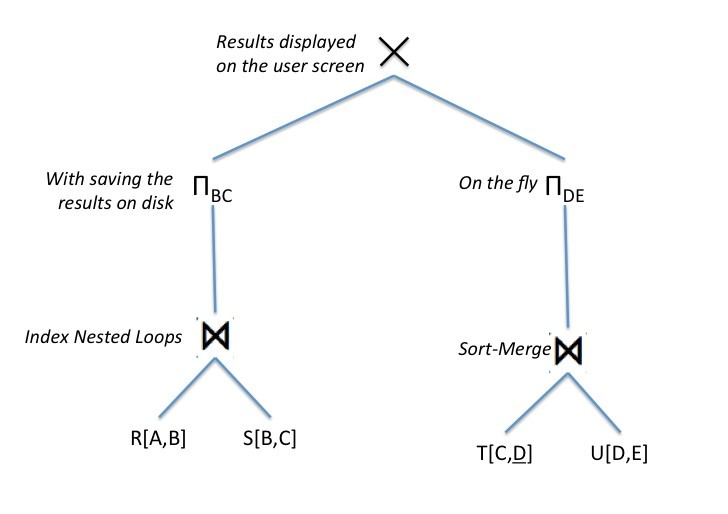
\includegraphics[scale=0.5]{img1.jpg}
\centering
\caption{An Example of a Query Plan}
\end{figure}

\begin{figure}[h]
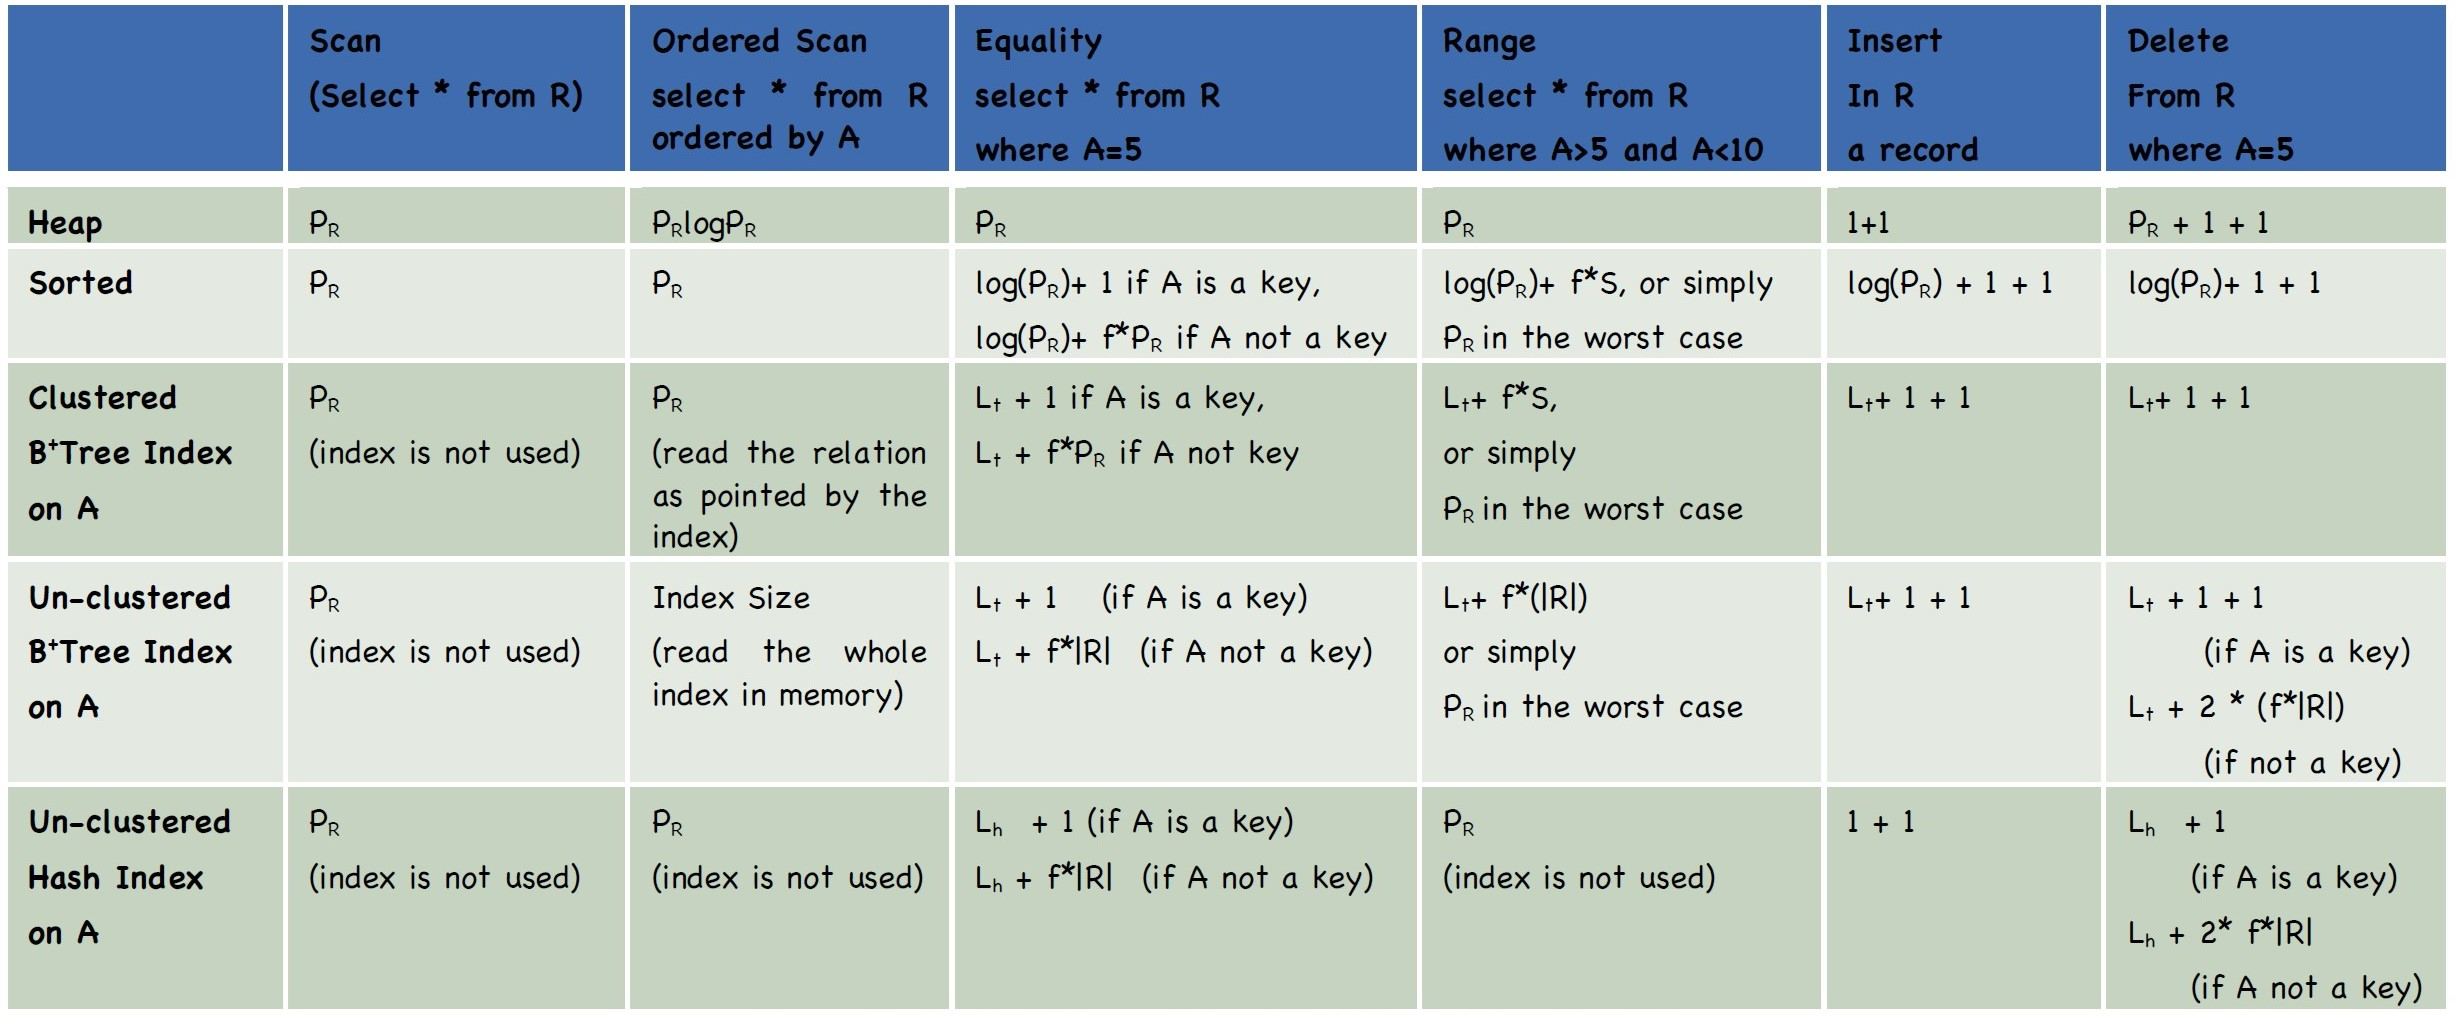
\includegraphics[scale=0.47]{img2.jpg}
\centering
\caption{Cost of operations that do not involve Joins}
\end{figure}

\end{document}
